\section{Background and Motivation}

The CESAR project aim to use low cost sensor kit to prototype applications using physiological signals related to heart rate, brain activity, oxygen level in blood to monitor sleep and breathing related illnesses, like Obstructive Sleep Apnea (OSA). Side effects of OSA do not only cause sleepiness during day time (which might affect daily chores), but also serious illnesses like diabetes and cardiac dysfunctions. Statistically speaking, it is estimated that about 25\% of the adult population in Norway has OSA, but only 10\% of them are diagnosed. A major problem with diagnosing OSA is polysomnography in \textit{sleep laboratories} \cite{cesar}. This is both really expensive and inefficient due to lacking capacity to perform sufficient tests with patients. Hence, the CESAR project aims to contribute to this situation with a low-cost Android and BiTalino based system to tackle these problems in a minimal invasive approach. 

The project has been developed by various people over the years, and the system has been divided into three parts (illustrated in Figure \ref{fig:parts}). The data acquisition part, the data streams dispatching part, and the application part. The first two parts are already implemented (summarized in the section below), thus, the last part is what we will be focusing throughout this thesis. 

\begin{figure}
    \centering
    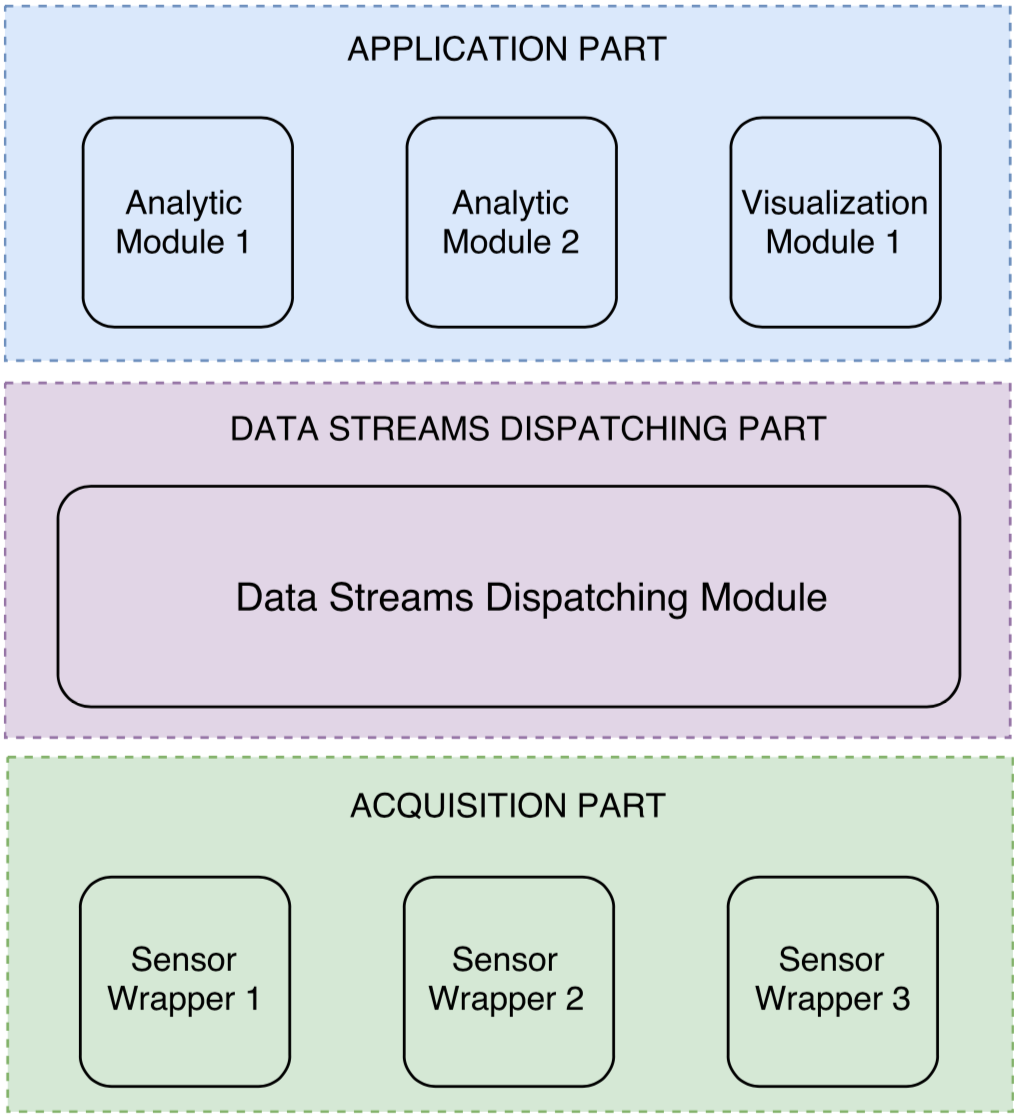
\includegraphics[width=0.5\textwidth]{images/parts.png}
    \caption{Structure of the project, separating functionality into three independent layers \cite{daniel}}
    \label{fig:parts}
\end{figure}
